\section{Challenges}

What challenges have occurred for this week?

Learning how to implement a list of options as well as type checking in Python was a very weird process. 
Python works off of the Ostrich Algorithm which is really funny to see, but horrifying when trying to work with particular types.

\begin{flushleft}
Another challenge we ran into that will be worked on in our next "sprint" is placing the traffic and placing moving obstacles on the road that is the traffic. I thought of placing spawnpoints on the street that a car Gameobject would spawn with the Sedan prefab and immediately assume moving on the road based on the default pathfinding function, but the current issue I'm running into is attaching that to the new gameobjects and how to make them recognize eachother as obstacles. The car could move, but it would just phase through the other cars, and the main car that will be caring about the end goals has a different function from the spawned in cars that I'll have to figure out if there's a more efficient way to script that or that I'll just continue with another script and worry about efficiency later.
\end{flushleft}

\begin{figure}[!ht]
    \centering
    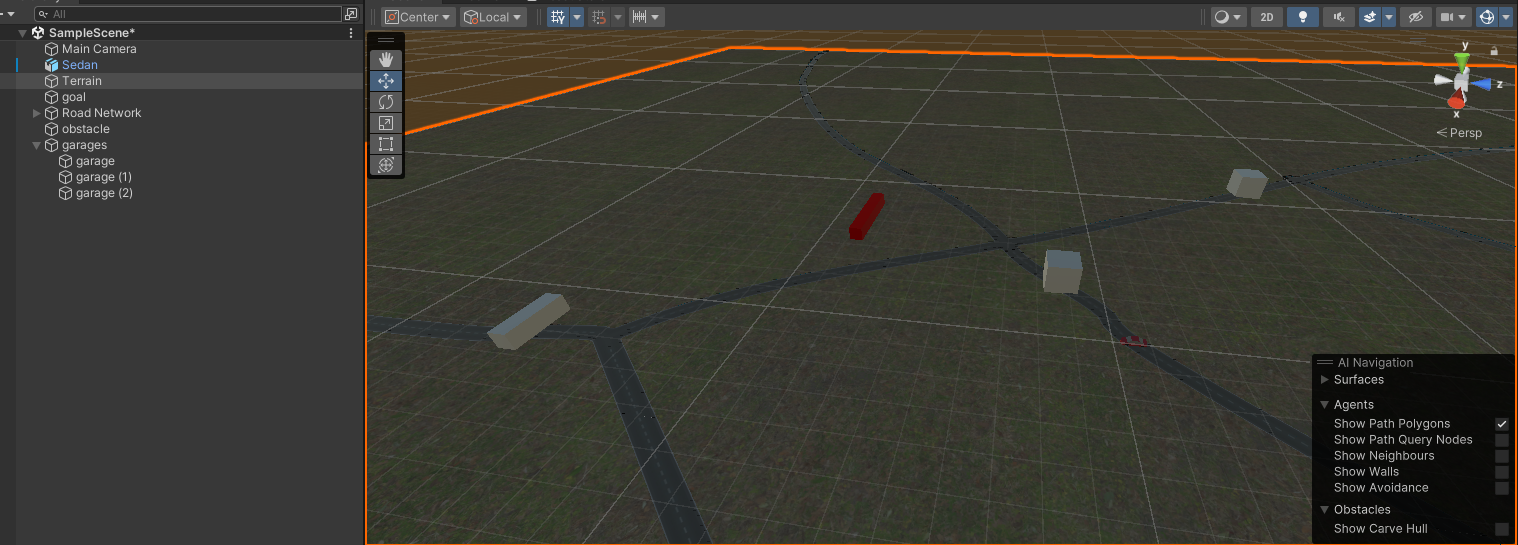
\includegraphics[width=10cm]{../Images/Update4/Garages.png}
       \caption{The grey boxes that are on the road, currently titled "garages", are the spawnpoints for cars.}
           \label{Fig: Bake Mesh Settings}
\end{figure}

\begin{flushleft}
The long red rectangle in the distance is an obstacle object I was testing with blocking the road and seeing where the car goes, which was how I found out that the car will keep going down a road regardless of obstacles.
\end{flushleft}